\chapter{Einleitung}

Im allgemeinen Sprachgebrauch wird unter {\bf Signal} ein Zeichen verstanden, mit dem eine Nachricht übertragen wird oder ein Verhalten, das eine Information übermittelt. Durch die Geophysik - aber auch durch andere Natur- oder Ingenieurwissenschaften - werden physikalische Messgrößen genutzt, um den Untersuchungsgegenstand zu analysieren. In einer physikalische Messgröße ist ein Signal vorhanden, wenn sie das Auftreten eines interessierenden Phänomens anzeigt.\\\\
Betrachtet man z.B. flächenhafte Messungen der Schwerebeschleunigung, so kann ein Signal ein Schwereminimum oder -maximum sein. Ein Signal kann aber auch ein Trend in den Messdaten sein, der eine räumliche Änderung der Tiefe des Grundgebirges anzeigt. Mit einem Seismometer wird die  Bewegung eines Massenpunktes, meistens in Form eine Spannung, aufgezeichnet. Trifft eine seismische Welle, die durch ein Erdbeben oder eine Sprengung angeregt werden kann, am Ort des Seismometers ein, wird ein Spannung induziert. In der Messgröße tritt ein Signal auf, das die seismische Welle beschreibt. In der Reflexionsseismik werden die Signale, d.h. die Wellenformen, die eine reflektierte Welle anzeigen, wavelet (\textsl{kleine Welle}) genannt.\\

Ein Massenpunkt ist aber nie komplett in Ruhe, z.B. weil menschliche Tätigkeiten mit Bewegungen verbunden sind, die zur ständigen Ausbreitung seismischer Wellen in der Erde führen. Interessiert man sich für Erdbeben, so ist die Registrierung einer durch das Erdbeben angeregten seismischen Welle das Signal, genauer das {\bf Nutzsignal}. Im Gegensatz dazu sind dann anthropogen erzeugte Wellen {\bf Störsignale}, die das eigentlich interessierende Signal überlagern. Interessiert man sich dagegen für die anthropogen erzeugten seismischen Wellen, um die Quellen oder auch den Untergrund zu untersuchen, so sind die durch das Erdbeben angeregten seismischen Wellen Störsignale und das eigentliche Signal oder das Nutzsignal sind die anthropogen hervorgerufenen seismischen Wellen. Ein Störsignal zeigt das Auftreten eines nicht interessierenden Phänomens an. Es hängt also von dem jeweiligen Untersuchungsgegenstand ab, was Signal und was Störsignal ist.\\
Wird eine andauernde Unruhe registriert, spricht man auch von {\bf Rauschen}, das auch von dem Messgerät selbst erzeugt werden kann. In Abhängigkeit von dem Ziel der Untersuchung, kann das Rauschen Nutz- oder Störsignal ist.  Rauschen ist also nicht immer Störsingal. Rauschen ist Nutzsignal, wenn Eigenschaften des Rauschens untersucht werden sollen. Das ist z.B. der Fall, wenn ruhige Standorte für empfindliche Messgeräte gesucht werden oder durch Wellen im Ozean erzeugtes seismischen Rauschen, die sogenannte Meeresmikroseismik, untersucht wird. Rauschen kann auch genutzt werden, um den Untergrund zu untersuchen. Dazu sind in den vergangenen Jahren verschiedene Verfahren entwickelt worden (Mikrozonierung, ambient noise). Seismische Unruhe kann auch durch Vulkane, Verwerfungen oder Fluidbewegungen im Untergrund erzeugt werden. Man spricht von vulkanischem oder nicht-vulkanischem Tremor, der Rückschlüsse auf den Zustand des anregenden Systems erlaubt und deshalb zunehmend untersucht wird.\\
Generell überlagern sich Nutz- und Störsignale in der betrachteten physikalischen Messgröße. Aufgabe der {\bf Signalverarbeitung} ist es, das Nutzsignal wahrnehmbar - meistens sichtbar - zu machen und seine Eigenschaften zu bestimmen. Mitunter soll das Signal auch hörbar oder fühlbar gemacht werden.\\
Ein Signal kann eine Funktion des Ortes oder der Zeit sein. Im Falle der erwähnten Schweremessung ist das Signal eine Funktion des Ortes, ein Seismometer liefert dagegen eine Funktion der Zeit.\\

Man unterscheidet weiter zwischen \textbf{analoger Signalverarbeitung} und \textbf{digitaler Signalverarbeitung}. Im Fall der analogen Signalverarbeitung wird das Signal durch mechanische oder elektrische Apparate wahrnehmbar gemacht. Beispiele für analoge Signalverabeitung ist z.B. analoges Radio oder Fernsehen. Empfangene elektromagnetische Wellen werden gefiltert und verstärkt, um das Nutzsignal möglichst ungestört wahrnehmbar zu machen. Ein Seismometer mit einer analogen Registierung ist ebenfalls ein Beispiel für analoge Signalverarbeitung: Anteile der Bodenbewegung werden herausgefiltert, verstärkt und als Funktion der Zeit registriert. Zur analogen Registrierung von Seismogrammen wurde Ende des 19. Jahrhunderts bis Mitte des 20. Jahrhunderts die Bodenbewegung mit einer Nadel in eine auf Papier aufgebrachte Rußschicht gekratzt, verschiedene Mechaniken und Massen wurden genutzt um das registrierte Signal zu \textit{filtern}. Später wurden Tonbänder verwendet, um die Ausgangsspannung des Seismometers analog zu speichern. Ein Feuermelder, der bei Auftreten von Rauch ein akustisches Signal gibt, ist ebenfalls ein Beispiel für analoge Signalverarbeitung. Anhand dieser Beispiele wird deutlich, dass elektronische oder mechanische Messgeräte generell als Beispiele analoger Signalverarbeitung dienen können.\\\\
Bei der digitalen Signalverarbeitung werden digitale Wertereihen, also Zahlenkolonnen, mit mathematische Methoden bearbeitet. Digitale Signalverarbeitung gibt es nicht erst seit der Einführung von Computern. Rechnen mit Messwerten, um eine Messgröße besser zu bewerten oder interpretiert zu können, gibt es seit der Antike. Anhand von Auflistungen der Warenbestände zu einer bestimmten Zeit kann geprüft werden, ob die Warenbestände einen bestimmten Wert unterschreiten, um sie nachzubestellen. Wenn die entsprechenden Zahlen den Schwellwert unterschreiten tritt ein Signal auf, dass dann eine Aktion zur Folge hat. Auch die regelmäßige Positionsbestimmung auf See, eine darauf beruhende Vorhersage des Kurses, die gegebenenfalls eine Kursänderung zur Folge hat, wenn das Ziel mit dem gegenwärtigen Kurs nicht erreicht wird, kann als Beispiel digitaler Signalverabeitung verstanden werden.\\

Mit dem Einsatz von Computern hat die digitale Signalverarbeitung eine enorme Verbreitung gefunden. Geophysikalische Beispiele sind die \textit{common mid point} Sta\-pelung (CMP-Stapelung) in der Reflexionsseismik, die digitale Filterung seismischer, seismologischer, gravimetrischer oder magnetischer Daten, die Bestimmung der Impedanz im Fall elektromagnetischer oder magnetotellurischer Messungen oder auch die Bearbeitung von GPS Signalen zur Positionsbestimmung. Auch die Berechnung der Eigenfrequenzen der Erde anhand von Amplitudenspektren seismologischer Aufzeichnungen gehört zur digitalen Signalverarbeitung. Den geophysikalischen Anwendungen gingen historisch Anwendungen in der Elektrotechnik und der Kommunikationsverarbeitung voraus.\\

Vielfältige Beispiele der digitalen Signalverarbeitung finden sich in der Astrophysik, der Meteorologie, Ozeanographie, aber auch der Medizin oder Ökonomie: Elektrische Signale des Herzen (Elektrokardiogramm) oder des Gehirns (Elektorencephalogramm) oder auch Börsenkurse werden digital bearbeitet und analysiert.\\
Die Enstehung der modernen mathematischen Grundlagen der Signalverarbeitung in der 1. Hälfte des 20. Jahrhunderts ist eng mit dem Wirken von Norbert Wiener und Andrej Kolmogorov verbunden. In der Geophysik haben z.B. Enders Robinson und Sven Treitel Wesentliches auf dem Gebiet der digitalen Signalverarbeitung geleistet. Im folgenden werden einführende Bücher zur digitalen Signalverarbeitung empfohlen.

\subsection*{Literatur Empfehlungen}
Andel, J., 1984. Statistische Analyse von Zeitreihen. Akademie-Verlag Berlin.\\\\
Brockwell, P.J., Davis, R.A., 1987. Time Series: Theory and Methods. Springer.\\\\
Box, G.,  Jenkins, G., 1970. Time series analysis: Forecasting and control. Holden-Day, San Francisco.\\\\
Buttkus, B., 1991. Spektralanalyse und Filtertheorie. Springer.\\\\
Karl, J.H., 1989. An Introduction to Digital Signal Processing. Academic Press.\\\\
Marple, S.L., 1987. Digital Spectral Analysis with Applications. Prentice-Hall.\\\\
Marsal, D., 1979. Statistische Methoden für Erdwissenschaftler. Schweizerbart’sche Verlagsbuchhandlung.\\\\
Press, W.H. et al., 1986. Numerical Recipes. Cambridge University Press.\\\\
Robinson, E.A., Treitel, S., 1980. Geophysical Signal Analysis. Prentice-Hall.\\\\
Silvia, M.T., Robinson, E.A., 1979. Deconvolution of Geophysical Time Series in the Exploration for Oil and Natural Gas. Elsevier.
 
\section{Geophysikalischen Signalanalyse}
Am Anfang einer geophysikalischen Untersuchung steht die Aufgabenstellung, aufgrund derer eine geeignete Messung durchgeführt wird. Diese liefert eine kontinuierliche Meßgröße, die nach einer Diskretisierung - meistens mit einem Analog-Digital-Wandler - in Form einer diskreten Wertereihe vorliegt. Die nächste Aufgabe ist das Datenmanagement, das dem Nutzer die Daten in geeigneter Form zur Verfügung stellt. Dann schließt sich die digitale Signalverarbeitung an, der eine Modellierung oder Inversion der Daten folgen kann. Schließlich werden die Ergebnisse interpretiert und entsprechend dokumentiert.\\

Liegen nur wenige Messdaten vor, ist das eine wichtige, aber relative einfache Aufgabe. Allerdings werden in der Geophysik oft erhebliche Datenmengen verarbeitet (bis mehrere TByte). Dann stellt ist es eine Herausforderung, die Daten möglichst lückenlos und fehlerfrei von dem Messort zu einem Datenarchiv zu übertragen und dort sicher zu speichern. Im Fall permanenter seismologischer Stationen werden die Daten heute in realtime (Echtzeit) an Datenzentren wie GEOFON, ORFEUS oder IRIS übertragen, die sie dann auch dem Nutzer durch geeignete Portale zur Verfügung stellen. Für große Datenmengen wird dem Nutzer neuerdings auch Software zur automatischen Abfrage der Daten bereitgestellt. Wichtig ist, dass auch sogenannte Metadaten verwaltet werden, ohne die die Messwerte nicht interpretiert werden können. Diese enthalten den Ort der Messungen, den Namen des Messgerätes und dessen Eigenschaften, den Zeitpunkt der Messungen und weitere Informationen wie den Namen von Netzwerken oder Messkampagnen oder die Messbedingungen. Es muss deutlich werden: Wer hat wann, wo, mit welchen Gerät und welchen Einstellungen, unter welchen Bedingungen, was gemessen? Auch der Eigentümer der Daten und die Nutzungsbedingungen können in den Metadaten enthalten sein.\\

Die \textbf{digitale Signalverarbeitung} umfasst 1. die Darstellung der Daten, 2. die digitale Bearbeitung der Daten und 3. die Schätzung von Signalparametern. Diese Schritte können wiederholt, in beliebiger Reihenfolge und iterativ erfolgen, bis das Signal in der gewünschten Form dargestellt wird. Oft steht interaktive Software für die digitale Signalverarbeitung zur Verfügung. Im Fall großer Datenmengen oder Bearbeitungen in realtime werden die Bearbeitungsschritte zumindest teilweise automatisiert. Oft muss eine optimale Strategie für die Bearbeitung der Daten in vielen Versuchen entwickelt werden. Die automatische Bearbeitung der Daten (mitunter in realtime) ist eine aktuelle Herausforderung bei der Bearbeitung geophysikalischer Daten.

\newpage


\section{Graphische Darstellung von Wertereihen}
Für die Darstellung von Wertereihen gibt es sehr viele Möglichkeiten. Eine geeignete Darstellung der Messdaten ist für die erfolgreiche Interpretation der Messdaten entscheidend oder mitunter auch ausreichend. Im folgenden sollen einige Möglichkeiten erwähnt werden.\\[.5cm]
Darstellungen der Form $f(x)$:
\begin{itemize}
    \item Darstellung in Form von Linen, Punkten, Histogrammen oder auch Darstellungen in Abhängigkeit eines Winkels. Beispiele sind die Darstellung von Seismogrammen, Messungen der Temperatur in Abhängigkeit der Zeit oder Messungen der Schwerebeschleunigung auf einem Profil. 
  \end{itemize}
  Darstellungen der Form  $f(x,t)$: 
\begin{itemize}
\item
Ein Beispiel sind Seismogrammsektionen: an verschiedenen Orten auf einem Profil wurden Seismogramme gemessen. Mitunter werden die Flächen unter positiven bzw. negativen Phasen auch eingefärbt.
\end{itemize}
  \begin{figure}[h!]
  \centering
  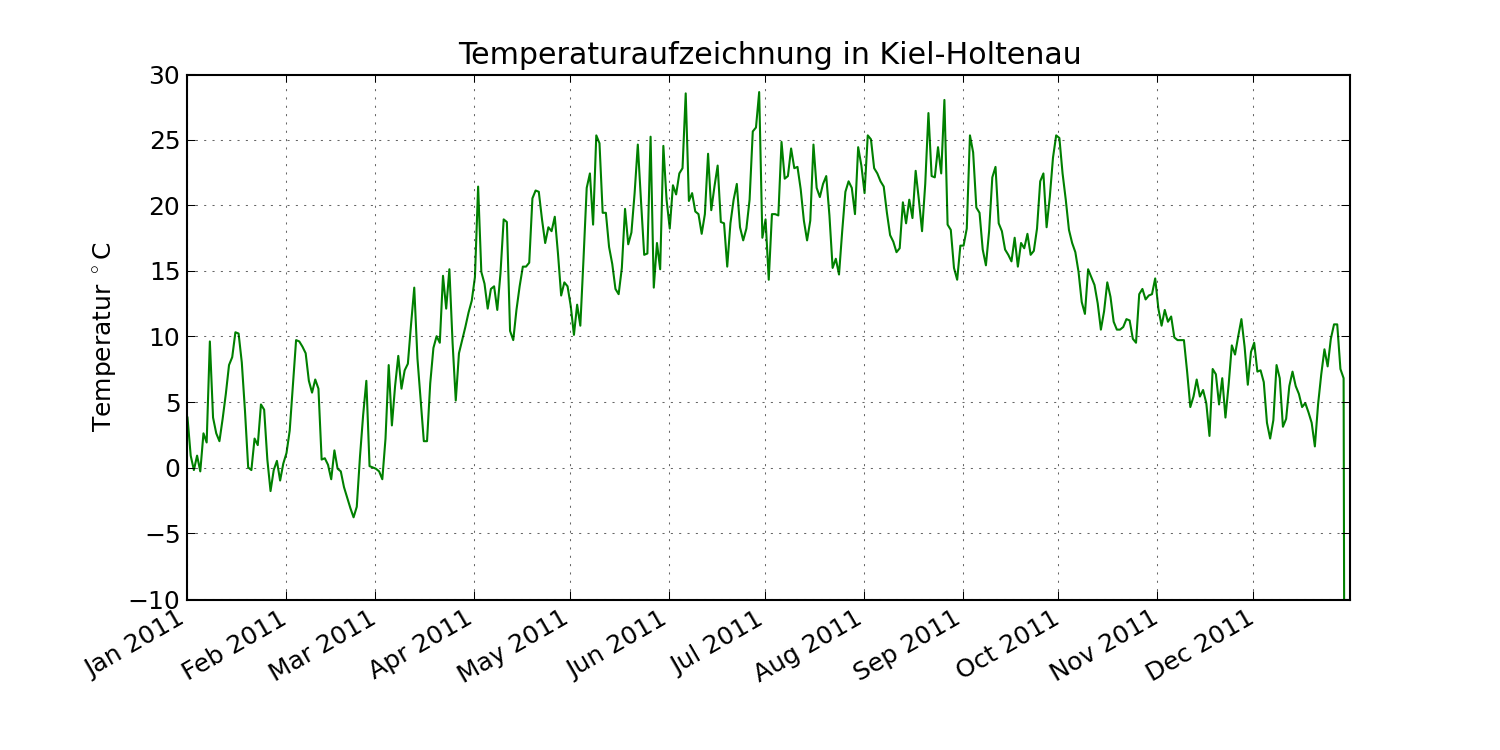
\includegraphics[width=.9\tw]{fig/03-Example-illustations/temperature-diagram_kiel}
  \caption{Darstellung einer Wertereihe der Art $f(x, t)$, Die Lufttemperatur im Jahresgang bei der Wetterstation Kiel-Holtenau.}
  \end{figure}
Darstellungen der Form $f(x,y)$:
\begin{itemize}
\item In 2D-Darstellungen wird der Messwert durch die Größe, Farbe oder Art der Symbole angezeigt. Ein Beipiel ist die Kennzeichnung von Epizentren durch Symbole, deren Größe proportional zur Magnitude ist. Statt einem kartesischen Koordinatensystem kann die Darstellung auch in anderen geographischen Projektionen oder in Polarkoordinaten erfolgen.
\item Konturplot (Isoliniendarstellung)
\item Einfärben von Bildpunkten. Eine Fotografie wird so dargestellt. Landkarten mit Höhenlinien sind eine Kombination dieser Darstellung mit einer Isoliniendarstellung.
\item 3D-Darstellungen von Oberflächen 
\item Darstellung in Polarkoordinaten: $f(r,\varphi)$
  \end{itemize}
Darstellungen der Form $ {\bf f}(x,y)$:
\begin{itemize}
\item
An den Orten $(x,y)$ werden Vektoren dargestellt, z.B. um Deformationen zu beschreiben.
\end{itemize}
Darstellungen der Form $f(x,y,z)$:
\begin{itemize}
\item Isooberflächen   
\item 3D-Plots mit Farbe, Größe oder Art der Symbole, die den Messwert $f$ anzeigen
\item Meistens werden 2D-Darstellungen der Messwerte auf ausgewählten, ebenen Schnitten bevorzugt. Beispiele sind Röntgenbilder.  
\item Es gibt Möglichkeiten der dreidimensionalen Darstellung, die meistens vor allem für die qualitative Bewertung sehr komplexer Datenstrukturen geeignet sind. 
  \end{itemize}
  
\noindent Darstellungen der Form $f(x,y,t)$: \begin{itemize}
\item Liegen flächenhafte Messungen als Funktion der Zeit vor, eignet sich die Visualisierung mit Hilfe von Filmen. Alternativ kann auch eine Folge von Bildern dargestellt werden.  
  \end{itemize}
Darstellung der Form $f(x,y,z,t)$:
\begin{itemize}
\item Derartige Messwerte - z.B. ein Dreikomponenten-Seismogramm - können auf einfachere Darstellungen zurückgeführt werden, indem die Komponenten des Seismogramms einzeln dargestellt werden. Es sind aber auch Projektionen der Partikelbewegung auf 3 senkrechte Ebenen möglich, wobei die Zeit farblich gekennzeichnet werden kann.
\end{itemize}
Weiterhin wurden spezielle Plots z.B. für die Darstellung von Herdflächenlösungen in Form sogenannter \textit{beachballs} entwickelt. 

\section{Bearbeitung der Signaldaten}
Im Folgenden werden Beispiele für die digitale Bearbeitung der Daten genannt.
\begin{itemize}
\item Trendkorrekturen, andere Korrekturen z.B. Korrektur von Zeitfehlern, Identifizierung und Entfernen von Ausreißern. 
\item Stapelung von Signalreihen
\item Detektion von Signal
\item Inter- und Extrapolation im Zeit- oder Ortsbereich
\item Approximation auch Komprimierung der Signalreihe
\item Resampling des Signalreihe
\item Korrelation : Korrelationsanalyse bei Vibroseismik, Kreuzkorrelation
\item Filterung und Wichtung in der Signalreihe
\item Transformationen (z.B. Fouriertransformation zur Berechnung von Frequenz- und Phasenpektren)
\end{itemize}

\section{Schätzung von Signalparametern}
Oft werden die bearbeiteten Daten nicht nur graphisch dargestellt, sondern es werden auch Signalparameter geschätzt, die interpretiert werden können oder als Input für Inversionen zur Verfügung stehen. Beispiele für Signalparameter sind:
\begin{itemize}
\item Signal-Rausch-Verhältnis (SNR), aber auch andere Qualitätsmaße
\item Frequenzspektren
\item Übertragunsfunktionen von Messgeräten und deren Korrektur
\item Herd-Zeit-Funktionen:(Abstrahlung im Herd), Wellenform des angeregten Signals
\item Schätzung einfacher Signalparameter wie Laufzeiten (Signaldetektion), Amplituden, Halbwertsbreiten etc., aber auch Schätzung von Streuamplituden durch Rückprojektion in einen Modellraum z.B. CMP-Stapelung
\item Schätzung von ARMA-Parametern, Poles and Zeros, Amplitude bzw. Phase einer bestimmten vorgegebenen Frequenz, Dämpfungsparamtern elastischer Wellen, Phasen- oder Gruppengeschwindigkeiten dispersiver Signale, Polarisationsparamter elastischer Wellen (z.B. Azimut, Einfallswinkel, Elliptizität), Eigenfrequenzen
\item Vorhersagen, Vorhersagefehler
\item Mustererkennung, Bestimmung von Ähnlichkeiten (z.B. Auto- und Kreuzkorrelation)
\item Slowness (Zeit-Frequenz-Analyse, f-k Analyse)
  \end{itemize}


\section{Forwärts Modellierung und Inversion}
Während durch die Signalverarbeitung Parameter des Signals, z.B. seiner Form, geschätzt werden, werden durch Modellierung und Inversion Parameter eines phy\-sikalischen Modells geschätzt, mit denen die Messung möglichst gut erklärt werden kann. Ein Trend in einer P-Wellenlaufzeitmessung kann als Signal bezeichnet werden. Der Anstieg wäre dann ein Signalparameter der z.B. durch einen Halbraum mit einer bestimmten P-Wellengeschwindigkeit erklärt werden kann. Die P-Wellengeschwindigkeit ist der Parameter des physikalischen Modells - in diesem Fall eines Halbraums. Generell muss bei der Inversion zunächst eine geeignete Parametrisierung der relevanten gesteinsphysikalischen Parameter vorgenommen werden. Das geschieht allgemein durch Entwicklung nach Basisfunktionen, die ein-, zwei- oder auch dreidimensional sein können.  Weiter müssen für vorgegebene Parameter - Wichtungen der Basisfunktionen - theoretische Messwerte bestimmt werden können. Bei der Inversion werden dann durch eine möglichst effektive Strategie Parameter gesucht, die in einem gewissen Sinn optimal sind, beispielsweise die Fehlerquadratsumme zwischen gemessenen Werten und theoretischen Werten minimieren. Idealerweise werden noch mögliche Wertebereiche für die Parameter angegeben und Mehrdeutigkeiten untersucht.  

\section{Ablauf einer geophysikalischen Untersuchung}
Vor jeder geophysikalischen Untersuchung muss die Aufgabenstellung klar definiert werden. Die Messmethoden werden ausgewählt gegenüber der Aufgabenstellung und Genauigkeit. Sodann kann die Messungen durchgeführt werden.
Der zweite Schritt ist die Diskritisierung der Messergebnissen mit Hilfe der Analog-Digital-Umwandlung (A/D-Wandler) um eine diskritisierte Wertereihe (z.B. die Punktmessung der Schwerebeschlunigung). Anschliessend müssen die Daten organisiert werden - Lokationen müssen zugeordnet, und Zeiten ggf. korrogiert werden. Sind die Daten gemessen folgt im dritten Schritt bei einer geophysikalischen Untersuchung die Signalbearbeitung. Dabei können beispielhaft folgende Aktionen durchgeführt werden: 
\begin{itemize}
\item Visualisierung der Messgröße (Darstellung der Daten, Farbskala einführen)
\item Bearbeitung von Daten
\item Signalparameter abschätzen
\end{itemize}
Der nächste Schritt ist die Modellierung/Inversion der Daten (Physikalische Parameter, Vorwärtsmodellierung/Inversionsmodellierung). Im Anschluss können die Ergebnisse der geophysikalischen Untersuchung interpretiert werden.

